\documentclass[11pt]{beamer}
\usetheme{metropolis}


\usepackage[utf8]{inputenc}
\usepackage[english]{babel}
\usepackage{amsmath}
\usepackage{amsfonts}
\usepackage{amssymb}
\usepackage{graphicx}
\usepackage{url}

\usepackage{marvosym}
\usepackage[export]{adjustbox}
\usepackage[T1]{fontenc}

\begin{document}
    \author{Mirco Haug}
    \title{On linear layouts with SAT}
    \institute{Eberhard Karls Universität Tübingen}
    \date{\today}
    \begin{frame}
        \maketitle
    \end{frame}

    \begin{frame}{Contents}
        \tableofcontents
    \end{frame}

    \section{Motivation}\label{sec:motivation}

    \begin{frame}{What to do?}
        \begin{center}
            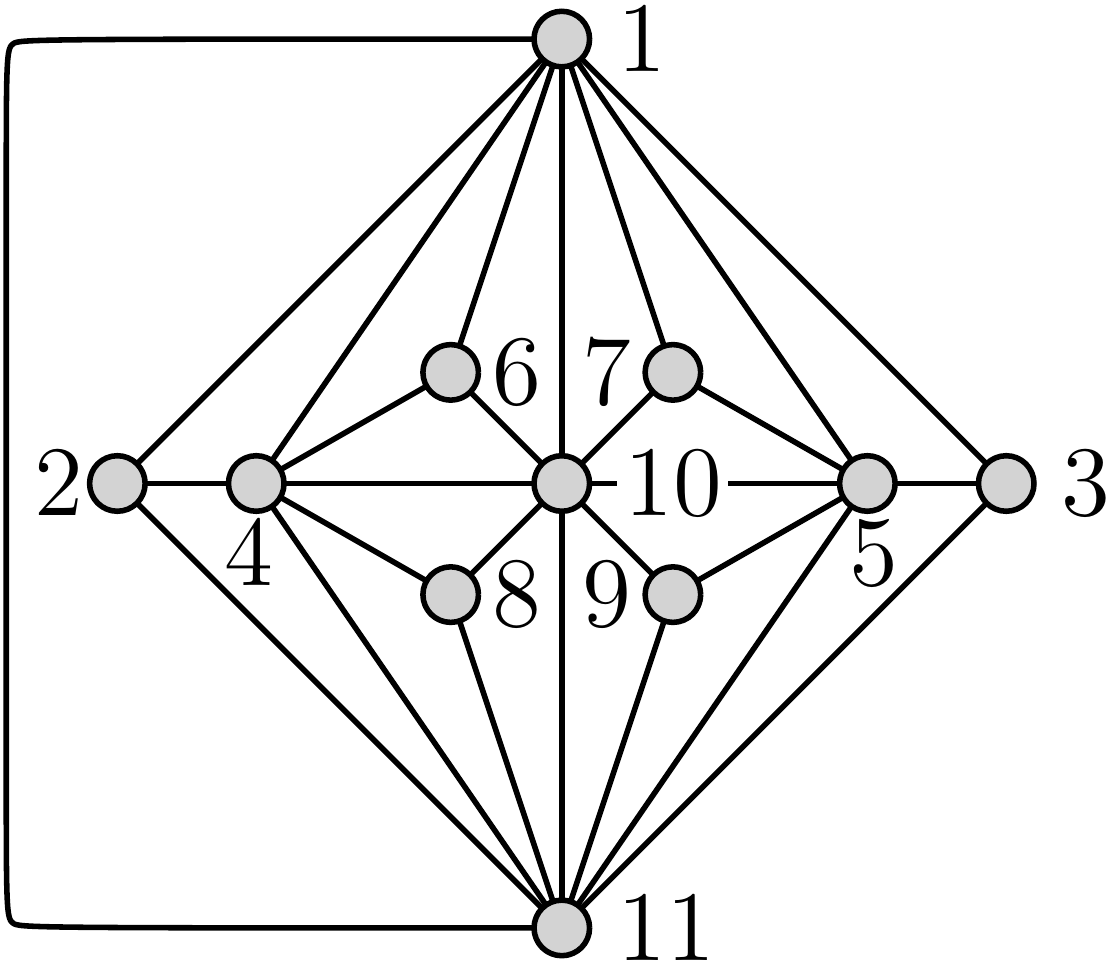
\includegraphics[width=0.4\linewidth,valign=c]{../_static/graphs/gh.png} $\Rightarrow$
            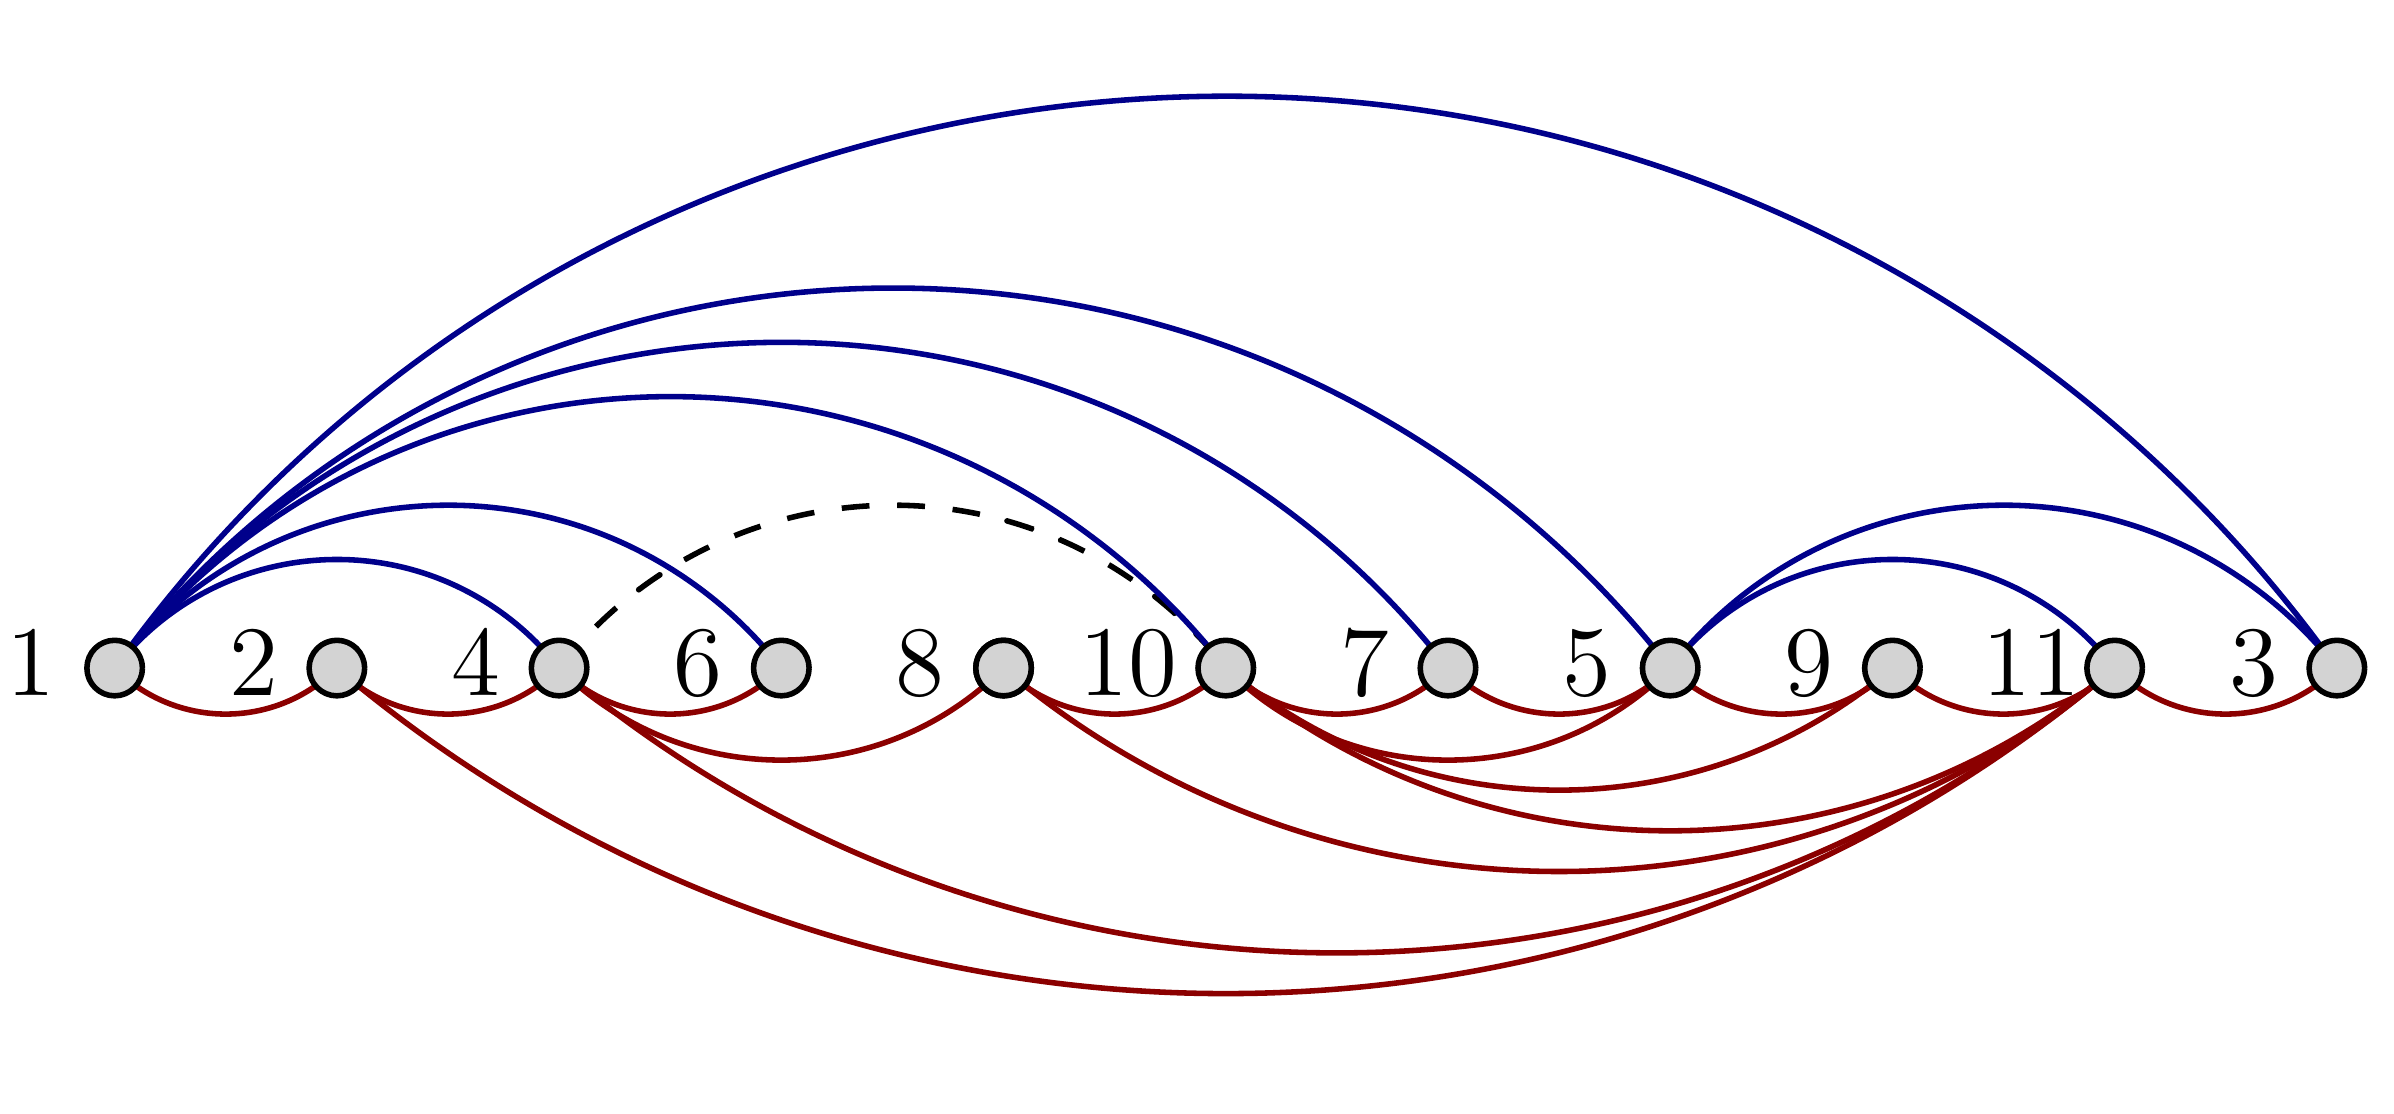
\includegraphics[width=0.54\linewidth,valign=c]{../_static/graphs/gh_stack.png}
        \end{center}
    \end{frame}

    \begin{frame}{The bookembedding problem}
        \begin{itemize}
            \item Multiple pages / Colors
            \item No crossings
            \item Node order
            \item Edge assignments
        \end{itemize}
    \end{frame}

    \begin{frame}
        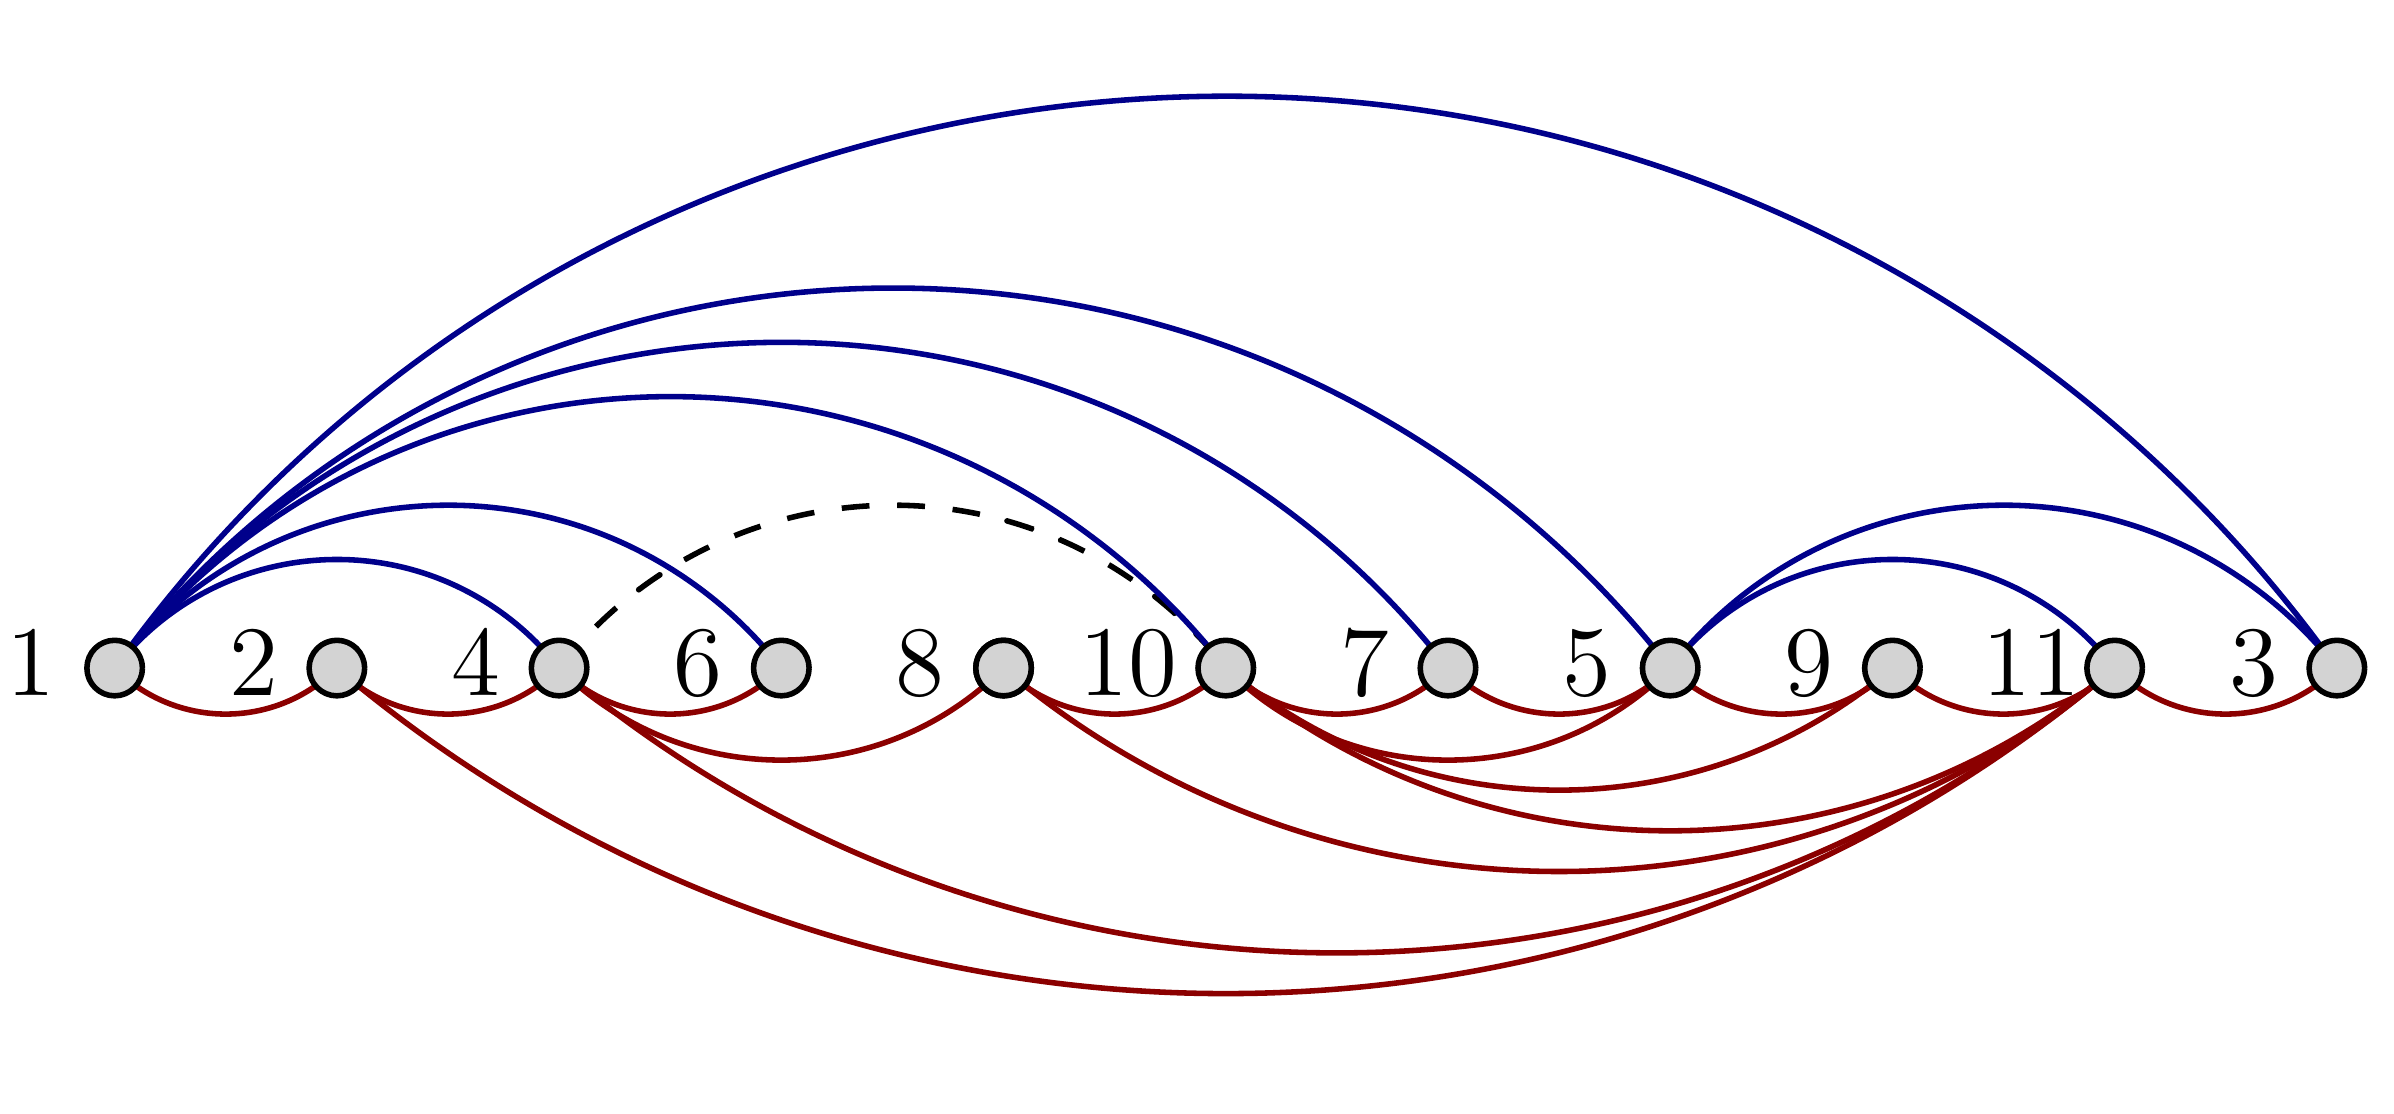
\includegraphics[width=\linewidth,valign=c]{../_static/graphs/gh_stack.png}
    \end{frame}

    \begin{frame}{Approach}
        \begin{itemize}
            \item Combinatoric explosion
            \item SAT solvers
            \item http://be.cs.arizona.edu
            \item Rather static
            \item Flexibility needed
            \item Old proof sketch of Yannakakis\cite{DBLP:conf/stoc/Yannakakis86}
        \end{itemize}
    \end{frame}

    \section{Theory}\label{sec:theoretical}
    \begin{frame}{Standart book embedding\cite{Bekos2015}}
        \begin{itemize}
            \item Node order $\sigma(n_1,n_2)$
            \item Edge assignment $\phi_{P1}(e_1)$
        \end{itemize}
    \end{frame}

    \begin{frame}{Constraints}
        \begin{itemize}
            \item EDGES\_ON\_PAGES
            \item EDGES\_SAME\_PAGES
            \item EDGES\_DIFFERENT\_PAGES
            \item \alert<2>{EDGES\_TO\_SUB\_ARC\_ON\_PAGES}
            \item EDGES\_FROM\_NODES\_ON\_PAGES
            \item \alert<2>{NODES\_PREDECESSOR}
            \item NODES\_REQUIRE\_ABSOLUTE\_ORDER
            \item NODES\_REQUIRE\_PARTIAL\_ORDER
            \item NODES\_FORBID\_PARTIAL\_ORDER
            \item NODES\_CONSECUTIVE
        \end{itemize}
    \end{frame}

    \section{Implementation}\label{sec:implementation}

    \begin{frame}
        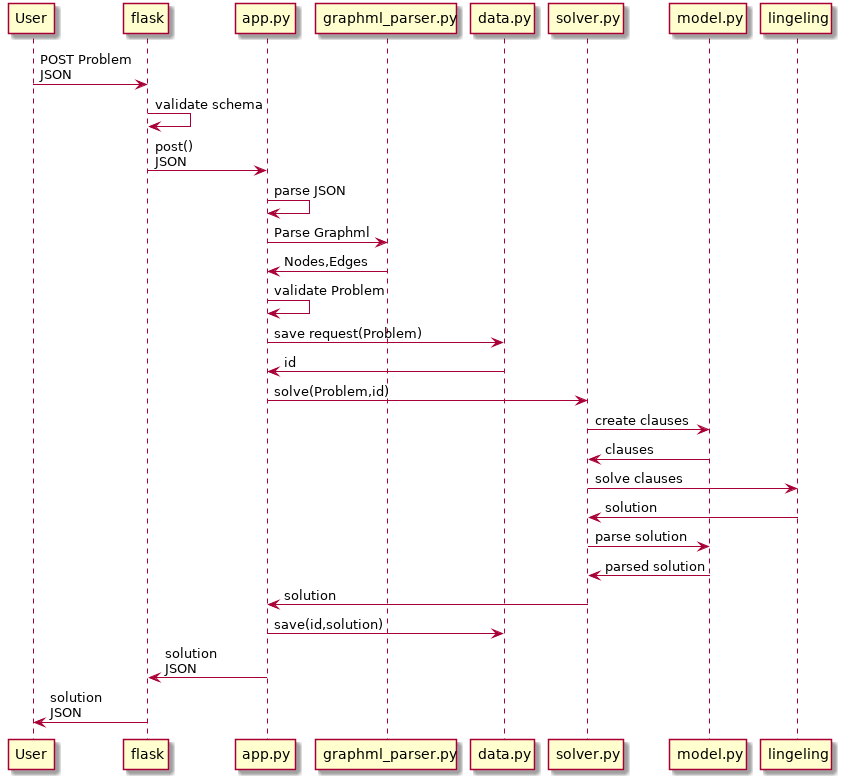
\includegraphics[height=\textheight]{flow.png}
    \end{frame}

    \begin{frame}{API $\Rightarrow$ Swagger UI}
        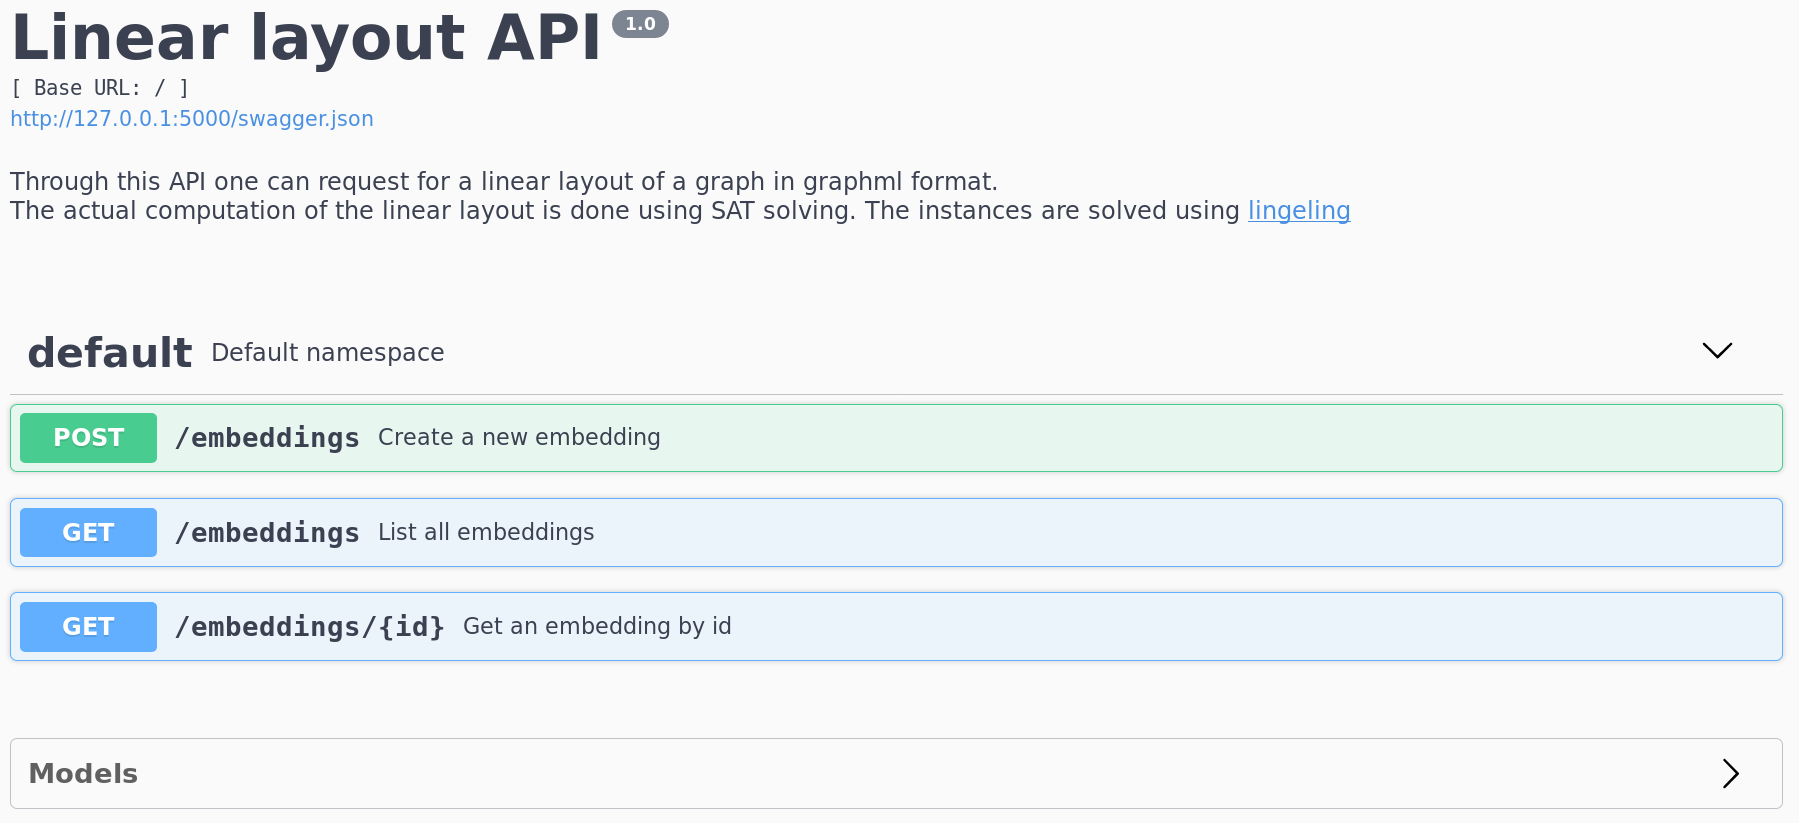
\includegraphics[width=\linewidth]{swagger-UI.png}
    \end{frame}

    \begin{frame}{Main classes}
        \begin{itemize}
            \item app.py
            \item model.py
            \item solver.py
        \end{itemize}
    \end{frame}


    \begin{frame}{app.py}
        \begin{itemize}
            \item Schema definition
            \item Deserialization
            \item Validate
        \end{itemize}
    \end{frame}

    \begin{frame}{solver.py}
        \begin{itemize}
            \item Glue
            \item Service interface
            \item Coordination
            \item Calls lingeling
        \end{itemize}
    \end{frame}

    \begin{frame}{model.py}
        \begin{itemize}
            \item Clause generation
            \item DIMACS Generation
            \item Parser for lingelinge result
        \end{itemize}
    \end{frame}


    \section{Demo}\label{sec:demo}
    \begin{frame}{Demo}
        \url{http://algo.inf.uni-tuebingen.de/linearlayouts/index.html\#or174}
    \end{frame}

    \begin{frame}{Bibliography}
        \bibliography{../references}
        \bibliographystyle{alpha}
    \end{frame}
\end{document}